\documentclass[../main.tex]{subfiles}
\begin{document}
本节的内容在大一的高等数学课中已经学过\cite[\S 9]{华工高数2009下},只是用本讲义的符号体系复述一遍基本内容。在这里我们需要强调的是,曲线和曲面都是3维欧几里得空间的点集。虽然我们将十分依赖这些点的在基本直角坐标系下的坐标来定义曲线、曲面,以及它们上的积分。但是,曲线和曲面是不依赖坐标系选择的几何对象。有关它们的相同事实在曲线坐标系下的表示,只需使用同一点的坐标变换性质就可以得到(见\S\ref{sec:II.5.2})。

以下我们默认所讨论的欧几里得空间$\mathcal{E}$是3维的,它的平移空间是$\mathcal{V}$,基本坐标系是$\left(O,\left\{\mathbf{\hat{e}}_i\right\}\right)$。为了文字叙述的简洁,我们默认一个$\mathcal{V}$中的平移向量的记号$\mathbf{x}\in\mathcal{V}$同时也表示其在基$\left\{\mathbf{\hat{e}}_i\right\}$下的坐标$\mathbf{x}=\left(x_1,x_2,x_3\right)^\intercal\in\mathbb{R}^3$。根据上下文,同字母的向量$\mathbf{x}$还可能对应欧几里得空间中的点$X$在基本坐标系下的坐标;说“点$\mathbf{x}$”就是在说点$X$。

\subsection{曲线积分}
若函数$C:\mathbb{R}\supset I\rightarrow\mathbb{R}^3$在连通区间$I$上分段连续可微,则以$\left(x_1,x_2,x_3\right)=C\left(u\right),u\in I$为参数方程的像集$\mathcal{C}\equiv C\left(I\right)$是$\mathcal{E}$中的一条\emph{可求弧长(rectifiable)}的曲线。例\ref{exp:II.4.7}已给出一个具体的例子。我们可以把映射$C$的分量函数记为$\mathbf{x}\left(u\right)=\left(x_1\left(u\right),x_2\left(u\right),x_3\left(u\right)\right)$。,则导数
\[
    \mathrm{D}C\left(u\right)\equiv\left(\frac{\mathrm{d}\mathbf{x}}{\mathrm{d}u}\right)=\left(\frac{\mathrm{d}x_1}{\mathrm{d}u},\frac{\mathrm{d}x_2}{\mathrm{d}u},\frac{\mathrm{d}x_3}{\mathrm{d}u}\right)^\intercal
\]
对应着$\mathcal{V}$中的一个向量$\mathbf{t}$,称为曲线$\mathcal{C}$在点$\mathbf{x}\left(u\right)$处的\emph{切向量(tangent vector)}。可定义$\mathbf{\hat{t}}\equiv\mathbf{t}/\left\|\mathbf{t}\right\|$为曲线$\mathcal{C}$在点$X$处的\emph{单位切向量(unit tangent vector)}。若把$\mathbf{\hat{t}}$画在点$X$处,它将会一个长度为1、方向朝曲线在$X$处切线方向的向量。

\begin{figure}[ht]
    \centering
    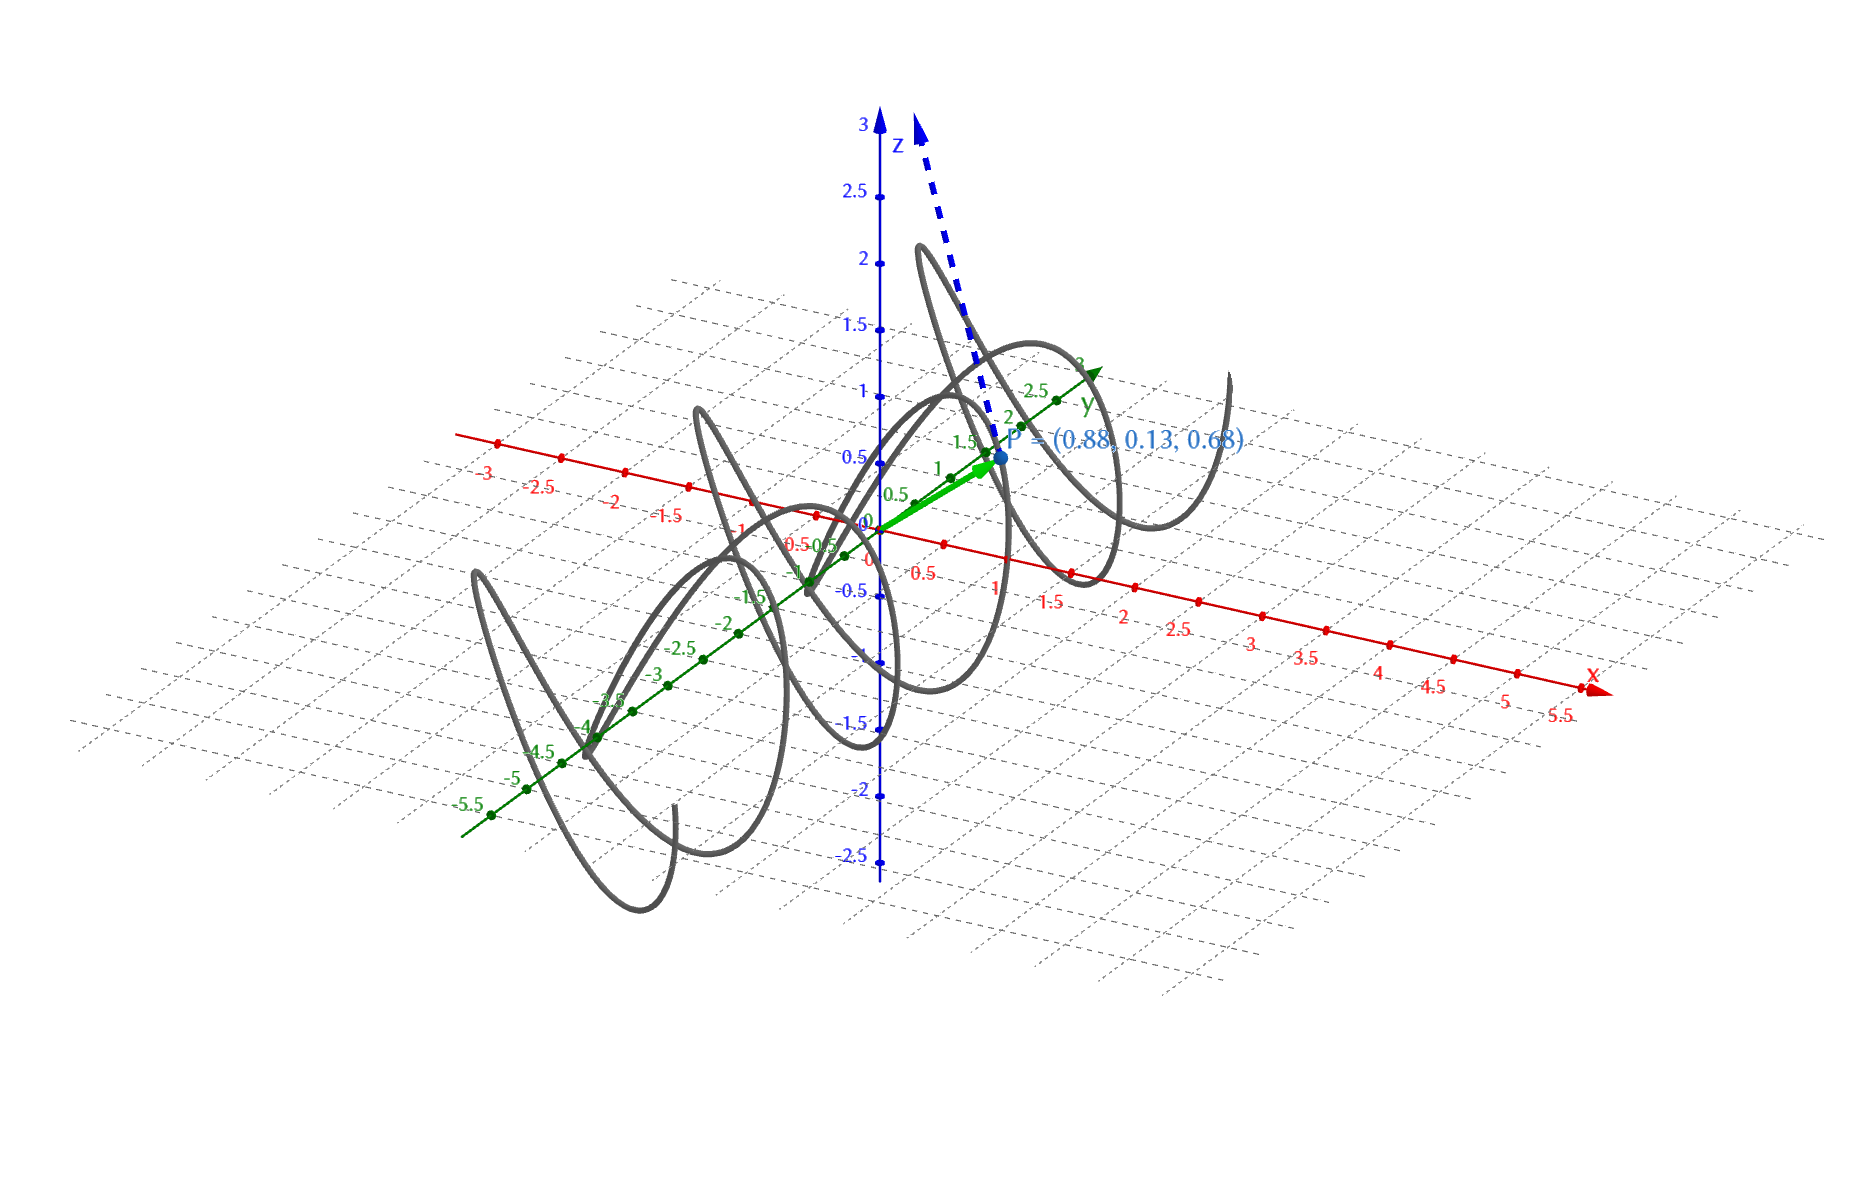
\includegraphics[width=\textwidth]{images/Tangent Vector.png}
    \caption{图中所示的是一条参数方程为$x\left(u\right)=\cos\left(2 u\right),y\left(u\right)=u/2,z\left(u\right)=\sin\left(3 u\right)$的曲线,在$u=0.25$处的点$P$的位置向量用绿色箭头表示,该处的切向量$\mathbf{t}$用蓝色虚线箭头表示。}
    \label{fig:II.5.3}
\end{figure}

曲线有两种微元。第一种微元是沿曲线的位移微元$d\mathbf{l}$,它作为$\mathcal{V}$中的向量,在$\left\{\mathbf{\hat{e}}_i\right\}$下的坐标是:
\[\mathrm{d}\mathbf{l}\equiv\mathbf{t}\mathrm{d}u=\left(\frac{\mathrm{d}x_1}{\mathrm{d}u},\frac{\mathrm{d}x_2}{\mathrm{d}u},\frac{\mathrm{d}x_3}{\mathrm{d}u}\right)^\intercal \mathrm{d}u\]
其实从记号惯例上说,$\mathrm{d}\mathbf{l}\equiv\mathrm{d}\mathbf{x}$,这里另用一个字母$l$是为了强调它的曲线微元角色。
第二种微元是沿曲线的弧长微元$\mathrm{d}l$,它就是位移微元的范数
\[\mathrm{d}l\equiv\left\|\mathrm{d}\mathbf{l}\right\|=\left\|\mathbf{t}\right\|\mathrm{d}u\]

曲线$\mathcal{C}$的\emph{弧长(arc length)}是曲线上的位移微元的总和:
\[L\left(\mathcal{C}\right)=\int_{\mathcal{C}}\mathrm{d}l=\int_I\left\|\mathbf{t}\right\|\mathrm{d}u\]
我们注意到,$\mathbf{t}\equiv \mathrm{D}C\left(u\right)$,因此,上式可写成
\[\int_\mathcal{C}\mathrm{d}\mathbf{x}=\int_I \left\|\mathrm{D}C\left(u\right)\right\|\mathrm{d}u\]
是一个按照$\mathbf{x}=C\left(u\right)$实施的积分换元公式。如果曲线的某个性质按照“单位弧长的量”$f:\mathbb{R}^3\subset\mathcal{C}\rightarrow\mathbb{R}^{3^n}$,其中$n=0,1,2,\cdots$分别表示该性质的值是标量、向量或二阶、……张量。则该性质对整条曲线的总和为对弧长微元的曲线积分\cite[\S 9.1]{华工高数2009下}
\[\int_\mathcal{C}f\left(\mathbf{x}\right)\mathrm{d}l=\int_I f\circ C\left(u\right)\left\|\mathbf{t}\left(u\right)\right\|\mathrm{d}u\]
例如,若曲线$\mathcal{C}$的线密度是函数$\rho\left(\mathbf{x}\right)$,则曲线$\mathcal{C}$的总质量
\[
    m\left(\mathcal{C}\right)=\int_\mathcal{C}\rho dl=\int_I\rho\left(\mathbf{x}\left(u\right)\right)\left\|\mathbf{t}\left(u\right)\right\|\mathrm{d}u
\]

\begin{figure}[ht]
    \centering
    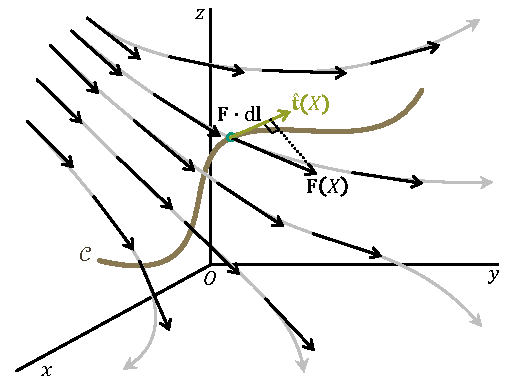
\includegraphics[width=0.5\textwidth]{images/line_integral.pdf}
    \caption{向量场$\mathbf{F}$在曲线$\mathcal{C}$上的积分,被积函数是向量场曲线上某点$X$的值与曲线在该点处的切方向上的投影$\mathbf{F}\cdot\mathrm{d}\mathbf{l}$。}
    \label{fig:II.5.4}
\end{figure}

如果曲线处于某向量场$\mathbf{F}:\mathbb{R}^3\supset\Omega\rightarrow\mathbb{R}^3$中,其中区域$\Omega\supset\mathcal{C}$,则曲线上各处的向量场对曲线的作用,是向量场在曲线切方向的投影(如图\ref{fig:II.5.4}所示),所以要拿同一处向量场的值与曲线的切向量点乘得到(在《高等数学》中称“对坐标的曲线积分”\cite[\S 9.2]{华工高数2009下}):
\[\int_\mathcal{C}\mathbf{F}\left(\mathbf{x}\right)\cdot \mathrm{d}\mathbf{l}=\int_I \mathbf{F}\circ C\left(u\right)\left\|\mathbf{t}\right\|\mathrm{d}u\]
例如,曲线$\mathcal{C}$是一个质点的运动轨迹,力场$\mathbf{F}\left(\mathbf{x}\right)$在这一过程中对该质点做的总功
\[W\left(\mathcal{C}\right)=\int_\mathcal{C}\mathbf{F}\cdot d\mathbf{l}=\int_I\mathbf{F}\left(C\left(u\right)\right)\cdot\mathbf{t}\left(u\right)du
\]

\subsection{曲面积分}
设函数$\mathbf{g}:\mathbb{R}^2\supset D\rightarrow\mathbb{R}^3$在由分段连续边界包围的连通区域$D$上连续可微,则以$\mathbf{g}\left(\mathbf{u}\right),\mathbf{u}\in D$为参数方程的像集$\mathbf{g}\left(D\right)$是$\mathbb{R}^3$中的一个可求面积的曲面,记为曲面$\mathcal{S}$。

当且仅当导数$\mathrm{d}_{\mathbf{u}=\mathbf{u}_0}\mathbf{g}\left(\mathbf{u}\right)$存在且满秩时,曲面$\mathcal{S}$在点$\mathbf{g}\left(\mathbf{u}_0\right)$处有切平面,或称曲面在此处是\emph{光滑的(smooth)}。此时
\[
    \left.\left(\frac{\partial \mathbf{g}}{\partial u_1}\times\frac{\partial \mathbf{g}}{\partial u_2}\right)\right|_{\mathbf{u}=\mathbf{u}_0}
\]
是曲面$\mathcal{S}$在点$\mathbf{g}\left(\mathbf{u}_0\right)$处的法向量,
\[
    \mathbf{\hat{n}}\equiv\left.\left(\frac{\frac{\partial \mathbf{g}}{\partial u_1}\times\frac{\partial\mathbf{g}}{\partial u_2}}{\left\|\frac{\partial\mathbf{g}}{\partial u_1}\times\frac{\partial\mathbf{g}}{\partial u_2}\right\|}\right)\right|_{\mathbf{u}=\mathbf{u}_0}
\]
是曲面$\mathcal{S}$在点$\mathbf{g}\left(\mathbf{u}_0\right)$处的单位法向量。

曲面有两种面微元:$d\boldsymbol{\sigma}=\left(\frac{\partial\mathbf{g}}{\partial u_1}\times\frac{\partial\mathbf{g}}{\partial u_2}\right)d\sigma_D$是有向曲面微元;$d\sigma=\left\|\frac{\partial\mathbf{g}}{\partial u_1}\times\frac{\partial\mathbf{g}}{\partial u_2}\right\|d\sigma_D$是面积微元。它们的关系是$d\boldsymbol{\sigma}=\mathbf{\hat{n}}d\sigma$。其中$d\sigma_D=du_1du_2$是参数域$D$上的二重积分微元。

曲面$\mathcal{S}$的面积
\[
    A\left(\mathcal{S}\right)=\int_\mathcal{S}d\sigma=\int_D\left\|\frac{\partial\mathbf{g}}{\partial u_1}\times\frac{\partial\mathbf{g}}{\partial u_2}\right\|d\sigma_D
\]

“单位面积的性质”$\mathbf{f}:\mathbb{R}^3\supset \mathcal{S}\rightarrow\mathbb{R}^n$在曲面$\mathcal{S}$上的总和是第一型曲面积分\cite[p.~165,定理9.4.1]{华工高数2009下}
\[
    \int_\mathcal{S}\mathbf{f}\left(\mathbf{g}\right)d\sigma=\int_D\mathbf{f}\left(\mathbf{g}\left(\mathbf{u}\right)\right)\left\|\frac{\partial\mathbf{g}}{\partial u_1}\times\frac{\partial\mathbf{g}}{\partial u_2}\right\|d\sigma_D
\]

“作用场”$\mathbf{h}:\mathbb{R}^3\supset\mathcal{S}\rightarrow\mathbb{R}^3$在曲面上的总作用是第二型曲面积分或对坐标的曲面积分\cite[\S 9.5]{华工高数2009下}
\[
    \int_\mathcal{S}\mathbf{h}\cdot d\boldsymbol{\sigma}=\int_D\mathbf{h}\left(\mathbf{g}\left(\mathbf{u}\right)\right)d\sigma_D=\int_\mathcal{S}\mathbf{h}\cdot\mathbf{\hat{n}}d\sigma
\]

\subsection{积分换元公式}
本科高等数学已接触过3重积分的情况\cite[\S 8.3“五”]{华工高数2009下}。

设$\mathcal{U}\subset\mathbb{R}^3$是由分段光滑边界包围的连通区域,则以参数方程$\mathbf{g}:\mathbb{R}^3\supset \mathcal{U}\rightarrow\mathbb{R}^3$规定的像集$\Omega=\mathbf{g}\left(\mathcal{U}\right)$是一个经过形变后的三维区域。当且仅当导数$\mathrm{d}_{\mathbf{r}=\mathbf{r}_0}\mathbf{g}\left(\mathbf{r}\right)$存在且满秩时,区域$\Omega$在点$\mathbf{r}_0$处是光滑的。此时
\[
    \left|\frac{\partial \mathbf{g}}{\partial r_3}\cdot\left(\frac{\partial\mathbf{g}}{\partial r_1}\times\frac{\partial\mathbf{g}}{\partial r_2}\right)\right|_{\mathbf{r}=\mathbf{r}_0}\equiv\left|\mathrm{det}\left(\mathrm{d}_{\mathbf{r}=\mathbf{r}_0}\mathbf{g}\left(\mathbf{r}\right)\right)\right|
\]
是由向量$\frac{\partial\mathbf{g}}{\partial r_1},\frac{\partial\mathbf{g}}{\partial r_2},\frac{\partial\mathbf{g}}{\partial r_3}$所搭成的平行六面体的体积。$\mathcal{U}$的体积元$dV_\mathcal{U}$与$\Omega$的体积元$dV_\Omega$之间的转换关系是
\[dV_\Omega=\left|\mathrm{det}\left(\mathrm{d}_{\mathbf{r}}\mathbf{g}\left(\mathbf{r}\right)\right)\right|
    dV_\mathcal{U}\]
区域$\Omega$的体积是
\[
    V\left(\Omega\right)=\int_\Omega dV_\Omega=\int_\mathcal{U}\left|\mathrm{det}\left(\mathrm{d}_{\mathbf{r}}\mathbf{g}\left(\mathbf{r}\right)\right)\right|dV_\mathcal{U}
\]
“单位体积的性质”$\mathbf{f}:\mathbb{R}^3\supset\mathcal{U}\rightarrow\mathbb{R}^3$在区域$\Omega$的总和为
\[
    \mathbf{F}\left(\Omega\right)=\int_\Omega\mathbf{f}\left(\mathbf{g}\right)dV_\Omega=\int_\mathcal{U}\mathbf{f}\left(\mathbf{g}\left(\mathbf{r}\right)\right)\left|\mathrm{det}\left(\mathrm{d}_{\mathbf{r}}\mathbf{g}\left(\mathbf{r}\right)\right)\right|dV_\mathcal{U}
\]
上式其实就是积分换元公式。

\subsection{积分定理}
给定函数$P,Q:\mathbb{R}^2\supset D\rightarrow\mathbb{R}$和边界分段光滑的单连通区域$D$,格林公式:
\[\int_D\left(\frac{\partial Q}{\partial x_1}-\frac{\partial P}{\partial x_2}\right)d\sigma_D=\int_{\partial D}Pdx_1+Qdx_2
\]
可改写成
\[
    \int_D\mathrm{curl}\mathbf{F}d\sigma_D=\int_{\partial D}\mathbf{F}\cdot d\mathbf{l}
\]
其中函数$\mathbf{F}:\mathbb{R}^2\supset D\rightarrow\mathbb{R}^2$在标准基下的坐标函数是$\mathbf{F}\left(\mathbf{x}\right)=\left(P\left(\mathbf{x}\right),Q\left(\mathbf{x}\right)\right)$。一般地,在标准基下函数$\mathbf{F}\left(\mathbf{x}\right)=\left(F_1\left(\mathbf{x}\right),F_2\left(\mathbf{x}\right)\right)$的旋度为
\[\mathrm{curl}\mathbf{F}=\frac{\partial F_2\left(\mathbf{x}\right)}{\partial x_1}-\frac{\partial F_1\left(\mathbf{x}\right)}{\partial x_2}\]
其中$\mathbf{x}=\left(x_1,x_2\right)$。

由格林公式又有,
\[
    \int_D\left(\frac{\partial F_1}{\partial x_1}+\frac{\partial F_2}{\partial x_2}\right)d\sigma_D=\int_{\partial D}-F_2dx_1+F_1dx_2
\]
该式可改写成
\[
    \int_D\mathrm{div}\mathbf{F}d\sigma_D=\int_{\partial D}\mathbf{F}\cdot d\boldsymbol{\sigma}
\]
一般地,在标准基下函数$\mathbf{F}\left(\mathbf{x}\right)=\left(F_1\left(\mathbf{x}\right),F_2\left(\mathbf{x}\right)\right)$函数$\mathbf{F}$的散度为
\[
    \mathrm{div}\mathbf{F}=\frac{\partial F_1\left(\mathbf{x}\right)}{\partial x_1}+\frac{\partial F_2\left(\mathbf{x}\right)}{\partial x_2}
\]
其中$\mathbf{x}=\left(x_1,x_2\right)$。

以上2维空间的例子可推广到3维。在标准基下函数$\mathbf{F}:\mathbb{R}^3\supset \mathcal{U}\rightarrow\mathbb{R}^3$的旋度
\[
    \mathrm{curl}\mathbf{F}=\left(\frac{\partial F_3}{\partial x_2}-\frac{\partial F_2}{\partial x_3},\frac{\partial F_1}{\partial x_3}-\frac{\partial F_3}{\partial x_1},\frac{\partial F_2}{\partial x_1}-\frac{\partial F_1}{\partial x_2}\right)^\intercal
\]
若函数$\mathbf{F}$在$D$上连纪可导且$\mathcal{U}$是开集则$\mathcal{U}$也是旋度函数$\mathrm{curl}\mathbf{F}\left(\mathbf{x}\right)$的定义域。

设$\mathcal{S}$是$\mathbb{R}^3$中的光滑曲面,$\mathbf{g}:\mathbb{R}^2\supset D\rightarrow\mathbb{R}^3$二阶连续可微,$D$是由分段光滑边界围成的单连通区域,$\mathbf{F}:\mathbb{R}^3\supset\mathcal{S}\rightarrow\mathbb{R}^3$是作用在曲面$\mathcal{S}$上的连续可微向量场,则有斯托克斯定理
\[\int_\mathcal{S}\mathrm{curl}\mathbf{F}\cdot d\boldsymbol{\sigma}=\int_{\partial \mathcal{S}}\mathbf{F}\cdot d\mathbf{g}
\]

在标准基下函数$\mathbf{F}:\mathbb{R}^3\supset \mathcal{U}\rightarrow\mathbb{R}^3$的散度
\[
    \mathrm{div}\mathbf{F}=\frac{\partial F_1}{\partial x_1}+\frac{\partial F_2}{\partial x_2}+\frac{\partial F_3}{\partial x_3}
\]
若函数$\mathbf{F}$在$D$上连纪可导且$\mathcal{U}$是开集则$\mathcal{U}$也是散度函数$\mathrm{curl}\mathbf{F}\left(\mathbf{x}\right)$的定义域。

设$\Omega$是$\mathbb{R}^3$中可数个简单区域的并集,由分段光滑边界围成。$\mathbf{F}:\mathbb{R}^3\supset\Omega\rightarrow\mathbb{R}^3$是存在于$\Omega$中的连续可微向量场,,则有高斯定理
\[
    \int_\Omega\mathrm{div}\mathbf{F}dV_\Omega=\int_{\partial \Omega}\mathbf{F}\cdot d\boldsymbol{\sigma}
\]
\end{document}